% Main loop of GSO-RL. Adapted from the CAEPIA 2026 slides.
\documentclass[border=0pt]{standalone}
% Shared preamble of the GSO-RL documentation figures.
% Compiled with latex (DVI) + dvisvgm; see ../build.sh.
\def\pgfsysdriver{pgfsys-dvisvgm.def}
\usepackage[T1]{fontenc}
\usepackage{lmodern}
\renewcommand{\familydefault}{\sfdefault}
\usepackage{amsmath, amssymb}
\usepackage{tikz}
\usetikzlibrary{positioning, shapes, arrows.meta, calc, fit, backgrounds}

% Palette
\definecolor{Purple}{RGB}{102, 0, 153}
\colorlet{ColMa}{green!50!black}   % macro-move M1
\colorlet{ColMb}{blue!70!black}    % macro-move M2
\colorlet{ColMc}{orange!85!black}  % macro-move M3
\definecolor{cGa}{RGB}{38, 166, 154}
\definecolor{cGb}{RGB}{229, 96, 76}
\definecolor{cGc}{RGB}{235, 165, 40}
\definecolor{cGd}{RGB}{125, 125, 215}
\definecolor{cGe}{RGB}{190, 60, 150}

% White background so figures stay readable in dark mode. The white rectangle lives on the
% "background" layer; figures draw their own backdrops on "behind", which sits above it.
\pgfdeclarelayer{behind}
\pgfsetlayers{background,behind,main}
\tikzset{every picture/.append style={show background rectangle,
  background rectangle/.style={fill=white, draw=none}, inner frame sep=8pt}}
% NOTE: with dvisvgm, text placed after a \color{...} group inside the same node is misplaced.
% Put differently coloured pieces of text in separate nodes.

\newcommand{\yes}{{\color{green!50!black}\checkmark}}
\newcommand{\nope}{{\color{red!70!black}$\boldsymbol{\times}$}}

% A region: guide with three concentric rings.  \guia[style]{x}{y}{color}{label}
\newcommand{\guia}[5][]{%
  \fill[#4!10, #1] (#2,#3) circle (1.05);
  \fill[#4!20, #1] (#2,#3) circle (0.7);
  \fill[#4!35, #1] (#2,#3) circle (0.35);
  \foreach \r in {0.35,0.7,1.05} \draw[#4, #1] (#2,#3) circle (\r);
  \fill[#4!80!black, #1] (#2,#3) circle (2pt);
  \node[#4!75!black, font=\scriptsize\bfseries, #1] at (#2,#3+1.22) {#5};
}

\begin{document}
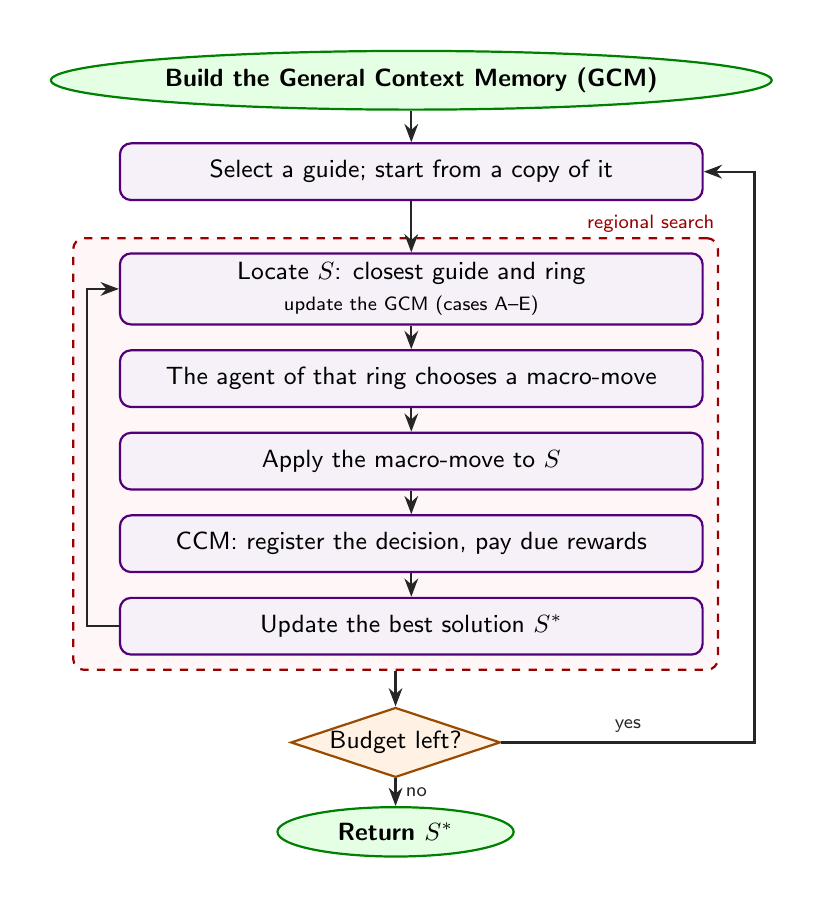
\begin{tikzpicture}[>=Stealth,
  process/.style={rectangle, draw=Purple!80!black, fill=Purple!6, thick, rounded corners,
                  minimum width=7.4cm, minimum height=0.72cm, align=center, font=\small},
  decision/.style={diamond, draw=orange!60!black, fill=orange!10, thick, aspect=3,
                   align=center, font=\small, inner sep=0.5pt},
  start/.style={ellipse, draw=green!50!black, fill=green!10, thick, minimum width=3cm,
                inner sep=3pt, font=\small\bfseries},
  arrow/.style={->, thick, gray!30!black}]
  \node (init) [start] {Build the General Context Memory (GCM)};
  \node (sel)  [process, below=0.4cm of init] {Select a guide; start from a copy of it};
  \node (loc)  [process, below=0.65cm of sel] {Locate $S$: closest guide and ring\\ \scriptsize update the GCM (cases A--E)};
  \node (act)  [process, below=0.3cm of loc] {The agent of that ring chooses a macro-move};
  \node (app)  [process, below=0.3cm of act] {Apply the macro-move to $S$};
  \node (rew)  [process, below=0.3cm of app] {CCM: register the decision, pay due rewards};
  \node (upd)  [process, below=0.3cm of rew] {Update the best solution $S^*$};
  \coordinate (lret) at ($(upd.west)+(-0.4,0)$);
  \begin{pgfonlayer}{behind}
    \node (loop) [draw=red!60!black, fill=red!3, thick, dashed, rounded corners,
                  inner sep=0.18cm, fit=(loc)(upd)(lret)] {};
  \end{pgfonlayer}
  \node[font=\scriptsize, red!60!black, anchor=south east, inner sep=1.5pt] at (loop.north east)
    {regional search};
  \coordinate (rx) at ($(loop.east)+(0.45,0)$);
  \node (dec) [decision, below=0.45cm of loop] {Budget left?};
  \node (end) [start, below=0.35cm of dec] {Return $S^*$};

  \draw[arrow] (init) -- (sel);
  \draw[arrow] (sel) -- (loc);
  \draw[arrow] (loc) -- (act);
  \draw[arrow] (act) -- (app);
  \draw[arrow] (app) -- (rew);
  \draw[arrow] (rew) -- (upd);
  \draw[arrow] (upd.west) -- (lret) |- (loc.west);
  \draw[arrow] (loop) -- (dec);
  \draw[arrow] (dec) -- node[right, font=\scriptsize] {no} (end);
  \draw[arrow] (dec.east) -- node[above, font=\scriptsize] {yes} (dec.east -| rx) |- (sel.east);
\end{tikzpicture}
\end{document}
